\section{广义逆矩阵}

\subsection{投影矩阵及其应用}

\begin{definition}[投影算子]
设 $\mathbb C^n=L\oplus M$,则对于任意 $x\in\mathbb C^n$ 有唯一分解 $x=y+z,\,y\in L,\,z\in M$.  称将 $x$ 变为 $y$ 的变换为沿着 $M$ 到 $L$ 的投影算子,记作 $P_{L,M}$,即:
\[P_{L,M}x=y\]
\begin{figure}[H]
    \centering
    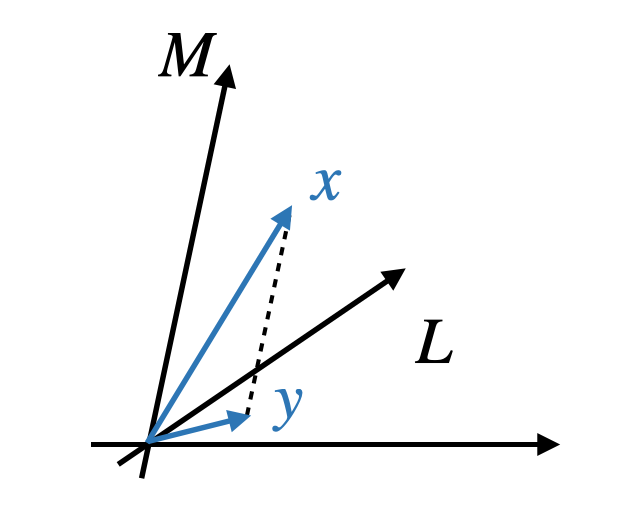
\includegraphics[width=0.2\linewidth]{figs/proj.png}
\end{figure}
\end{definition}

\begin{property}
$R(P_{L,M})=L,\,N(P_{L,M})=M$. 注意 $x-y\in M$.
\end{property}

\begin{definition}[投影矩阵]
投影算子 $P_{L,M}$ 在 $\mathbb C^n$ 的基 $(e_1,\ldots,e_n)$ 下的矩阵称为投影矩阵。
\end{definition}

\begin{lemma}
设 $A\in\mathbb C^{n\times n}$ 是幂等矩阵,即 $A^2=A$,则:
\[N(A)=R(I-A)\]
\end{lemma}
\begin{proof}
任取 $x\in N(A)$,则 $Ax=0$,则 $x=Ax+(I-A)x=(I-A)x\in R(I-A)$,因此 $N(A)\subset R(I-A)$;
任取 $y\in\mathbb C^n$,$A(I-A)y=(A-A^2)y=0$,故 $(I-A)y\in N(A)$,故 $R(I-A)\subset N(A)$;
综上,$N(A)=R(I-A)$.
\end{proof}

\begin{theorem}[投影与幂等]
矩阵 $P$ 为投影矩阵的充要条件是 $P$ 为幂等矩阵,即:
\[
    P_{n\times n}=P_{L,M}\iff P^2=P
\]
\end{theorem}
\begin{proof}
必要性:设 $C^n=L\oplus M$,则对于任意 $x\in\mathbb C^n$,存在唯一的分解 $x=y+z,\,y\in L,\,z\in M$.  于是 $P_{L,M}x=y$. 因此 $P_{L,M}^2x=P_{L,M}y=y=P_{L,M}x$,即 $P_{L,M}$ 是幂等的。

充分性:任意 $x\in\mathbb C^n$ 可分解为 $x=Px+(I-P)x$,根据引理知 $N(P)=R(I-P)$,又 $\mathbb C^n=R(P)\oplus N(P)$,所以这样的分解是唯一的,于是 $P=P_{R(P),N(P)}$.
\end{proof}

\noindent\textbf{计算方法}:取 $L$ 的一组基 $(q_1,\ldots,q_r)$ 和 $M$ 的一组基 $(q_{r+1},\ldots,q_n)$,则任意向量 $x\in\mathbb C^n$ 可表示为:
\[
    x=(q_1,\ldots,q_r,q_{r+1},\ldots,q_n)y=Qy
\]
于是:
\[
    P_{L,M}x=QI_ry=QI_rQ^{-1}x\implies P_{L,M}=QI_rQ^{-1}
\]
其中 $I_r$ 表示前 $r$ 个对角元为 1、其余为 0 的对角矩阵。

\begin{com}
可以看见上面的计算方法涉及到基的选取,但可以证明选取不同的基算出来的 $P_{L,M}$ 都是一样的。
假设另选一组基 $\bar Q_L=(\bar q_1,\ldots,\bar q_r)$ 和 $\bar Q_M=(\bar q_{r+1},\ldots,\bar q_n)$,设 $\bar Q_L=Q_LR_1,\,\bar Q_M=Q_MR_2$,则 $\bar Q=Q\text{diag}(R_1,R_2)$,于是:
\[
    \bar P_{L,M}=\bar Q I_r\bar Q^{-1}=Q\text{diag}(R_1,R_2)I_r\text{diag}(R_1^{-1},R_2^{-1})Q^{-1}=QI_rQ^{-1}=P_{L,M}
\]
可见 $P_{L,M}$ 与基的选取无关。
\end{com}

\begin{definition}[正交投影算子]
设 $L$ 是 $\mathbb C^n$ 的子空间,则沿着 $L^{\perp}$ 到 $L$ 的投影算子 $P_{L,L^{\perp}}$ 为正交投影算子,简记为 $P_L$.
\begin{figure}[H]
    \centering
    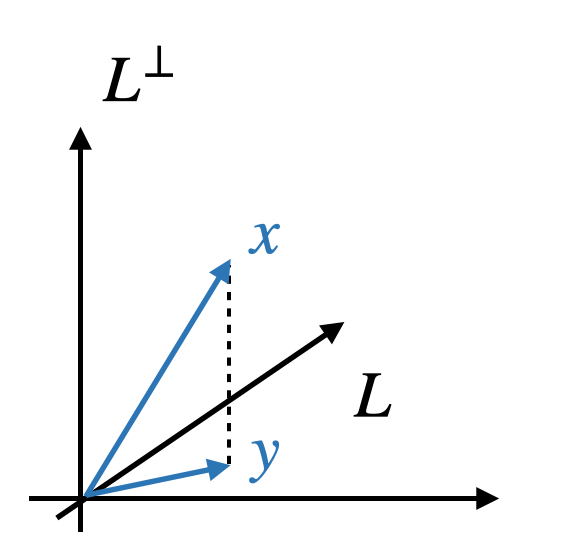
\includegraphics[width=0.2\linewidth]{figs/proj-o.png}
\end{figure}
\end{definition}

\begin{definition}[正交投影矩阵]
正交投影算子 $P_{L}$ 在 $\mathbb C^n$ 的基 $e_1,\ldots,e_n$ 下的矩阵称为正交投影矩阵。
\end{definition}


\begin{theorem}[正交投影与幂等 Hermite]
矩阵 $P$ 为正交投影矩阵的充要条件是 $P$ 为幂等 Hermite 矩阵。
\end{theorem}
\begin{proof}
必要性:若 $P$ 为正交投影矩阵,则根据上一节定理知它是幂等矩阵,于是 $R(I-P)=N(P)$。又 $R(P)\perp N(P)$,所以 $R(P)\perp R(I-P)$,因此对于任意 $x,y\in\mathbb C^n$,有:
\begin{align*}
    x^HP^H(I-P)y=0&\implies P^H(I-P)=0\implies P^H=P^HP\\&\implies P=(P^HP)^H=P^HP=P^H
\end{align*}
即 $P$ 是 Hermite 矩阵。

充分性:若 $P$ 是幂等 Hermite 矩阵,则根据上一节定理知它是投影矩阵 $P_{R(P),N(P)}$.  又由于 $P^H=P$,所以:
\[
    P_{R(P),N(P)}=P_{R(P),N(P^H)}=P_{R(P),R^\perp(P)}
\]
即 $P$ 是正交投影矩阵。
\end{proof}

\noindent\textbf{计算方法}:取 $L$ 的一组基 $X=(x_1,\ldots,x_r)$,$L^{\perp}$ 的一组基 $y=(y_1,\ldots,y_{n-r})$,则 $X^HY=Y^HX=O$.  根据上一节投影矩阵的计算方法知:
\[
    P_L=P_{L,L^\perp}
    =\left[\begin{array}{c:c}X&Y\end{array}\right]\;I_r\;\left[\begin{array}{c:c}X&Y\end{array}\right]^{-1}
    =\left[\begin{array}{c:c}X&O\end{array}\right]\left[\begin{array}{c:c}X&Y\end{array}\right]^{-1}
\]
由于:
\[
    \left[\begin{array}{c:c}X&Y\end{array}\right]^{H}\left[\begin{array}{c:c}X&Y\end{array}\right]=\left[\begin{array}{c}X^H\\\hdashline Y^H\end{array}\right]\left[\begin{array}{c:c}X&Y\end{array}\right]=\left[\begin{array}{c:c}X^HX&O\\\hdashline O&Y^HY\end{array}\right]
\]
于是:
\[
    \left[\begin{array}{c:c}X&Y\end{array}\right]^{-1}=\left[\begin{array}{c:c}(X^HX)^{-1}&O\\\hdashline O&(Y^HY)^{-1}\end{array}\right]\left[\begin{array}{c}X^H\\\hdashline Y^H\end{array}\right]=\left[\begin{array}{c}(X^HX)^{-1}X^H\\\hdashline(Y^HY)^{-1}Y^H\end{array}\right]
\]
因此:
\[
    P_L=\left[\begin{array}{c:c}X&O\end{array}\right]\left[\begin{array}{c:c}X&Y\end{array}\right]^{-1}=\left[\begin{array}{c:c}X&O\end{array}\right]\left[\begin{array}{c}(X^HX)^{-1}X^H\\\hdashline(Y^HY)^{-1}Y^H\end{array}\right]=X(X^HX)^{-1}X^H
\]

\begin{com}
同样的,正交投影矩阵的计算也与选取的基无关。假设有另一组基 $\bar X=(\bar x_1,\ldots,\bar x_r)$,设 $\bar X=XR$,则:
\begin{align*}
    \bar P_L&=\bar X({\bar X}^H\bar X)^{-1}{\bar X}^H=XR(R^HX^HXR)^{-1}R^HX^H\\
    &=XRR^{-1}(X^HX)^{-1}(R^H)^{-1}R^HX^H=X(X^HX)^{-1}X^H=P_L
\end{align*}
可见 $P_L$ 与基的选取无关。
\end{com}

\begin{remark}
由于 $X$ 是列满秩矩阵,根据下一节的内容可知 $X^+=(X^HX)^{-1}X$,所以 $P_L=XX^+$.
\end{remark}


\subsection{广义逆矩阵的存在、性质及构造方法}

\begin{definition}
\label{def:moore-penrose}
设矩阵 $A\in\mathbb C^{m\times n}$,若矩阵 $X\in\mathbb C^{n\times m}$ 满足如下四个 Penrose 方程:
\begin{align*}
    &AXA=A\tag{1}\label{1}\\
    &XAX=X\tag{2}\label{2}\\
    &(AX)^H=AX\tag{3}\label{3}\\
    &(XA)^H=XA\tag{4}\label{4}
\end{align*}
则称 $X$ 为 $A$ 的 Moore-Penrose 逆,记作 $A^+$.
若 $X$ 值满足上述四个方程中的第 $(i),(j),\ldots,(l)$ 个方程,则称 $X$ 为 $A$ 的 $\{i,j,\ldots,l\}$-逆,记作 $A^{(i,j,\ldots,l)}$,其全体记为 $A\{i,j,\ldots,l\}$.

如下为 1-逆的示意图:
\begin{figure}[H]
    \centering
    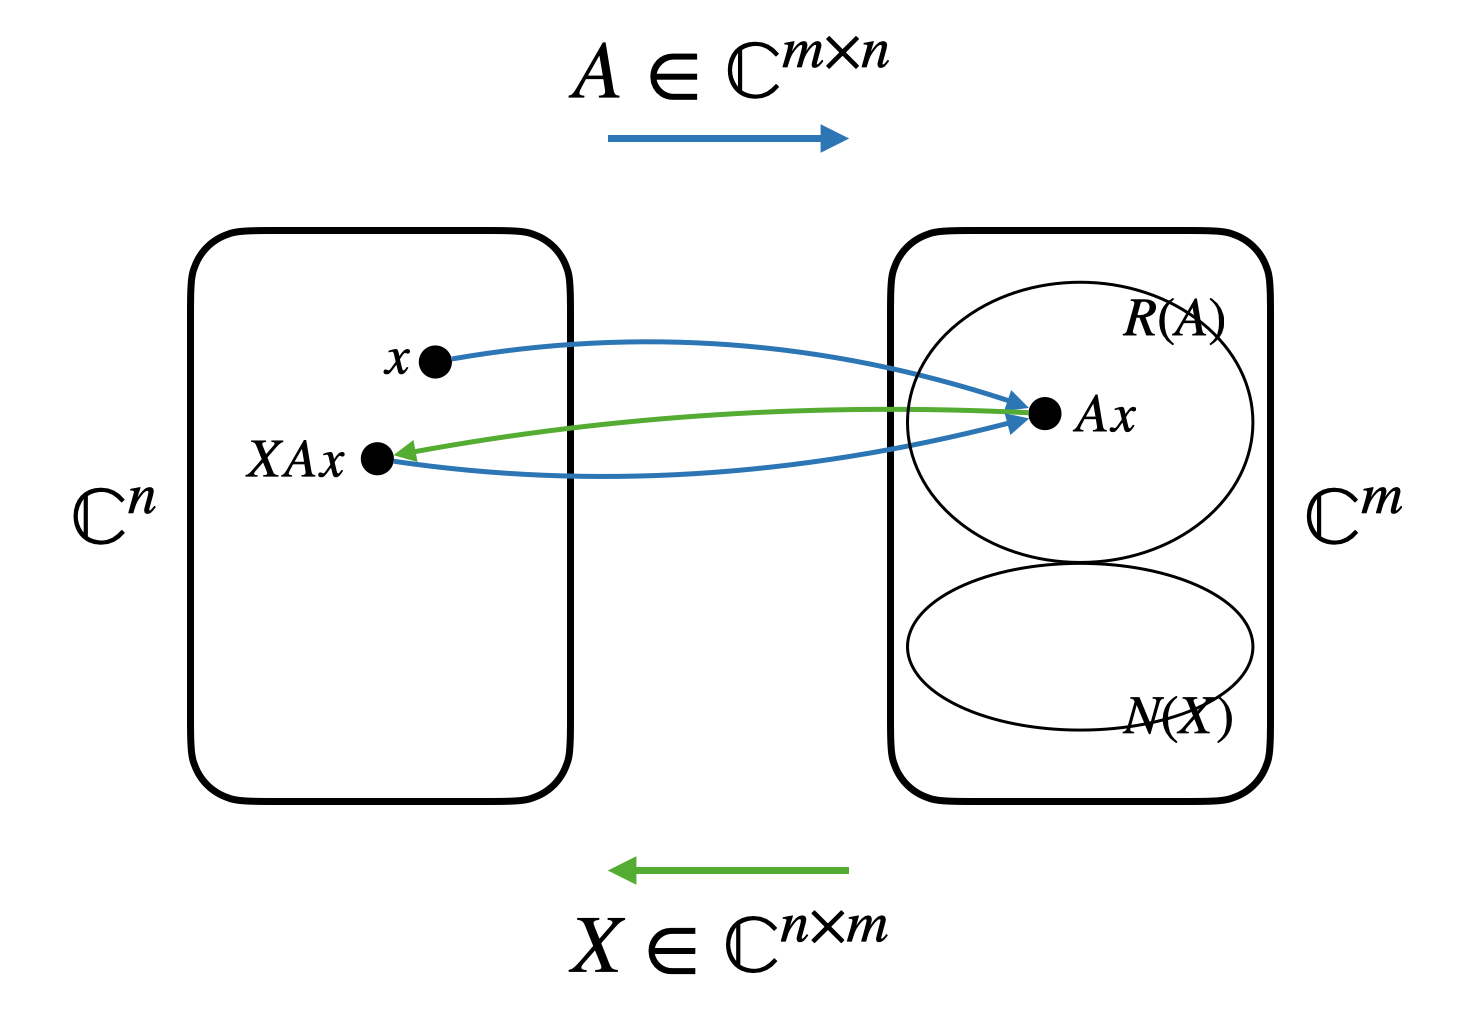
\includegraphics[width=0.5\linewidth]{figs/1inv.png}
\end{figure}
\end{definition}

\begin{theorem}
对任意 $A\in\mathbb C^{m\times n}$,$A^+$ 存在且唯一。
\end{theorem}
\begin{proof}
存在性。对 $A$ 做奇异值分解 $A=U\begin{bmatrix}\Sigma&0\\0&0\end{bmatrix}V^H$,取 $X=V\begin{bmatrix}\Sigma^{-1}&0\\0&0\end{bmatrix}U^H$,可以验证 $X$ 满足 $A^+$ 的四个条件。

唯一性。设 $X,Y$ 均是 $A^+$,则:
\begin{align*}
    Y&=YAY=Y(AY)^H=YY^HA^H=YY^H(AXA)^H\\&=YY^HA^H(AX)^H=Y(AY)^HAX=YAYAX=YAX\\
    X&=XAX=(XA)^HX=A^HX^HX=(AYA)^HX^HX\\&=(YA)^HA^HX^HX=(YA)^H(XA)^HX=(YA)^HXAX=(YA)^HX=YAX
\end{align*}
故 $X=Y$.
\end{proof}

\begin{remark}
上述定理的证明过程也给出了 $A^+$ 的一种基于奇异值分解的计算方法:
\[
    A=U\begin{bmatrix}\Sigma&0\\0&0\end{bmatrix}V^H\implies     A^+=V\begin{bmatrix}\Sigma^{-1}&0\\0&0\end{bmatrix}U^H
\]
\end{remark}

\begin{theorem}
\[
    \lim_{\delta\to0}(\delta^2I+A^HA)^{-1}A^H=A^+
\]
\end{theorem}
\begin{proof}
设 $A=U\begin{bmatrix}\Sigma&0\\0&0\end{bmatrix}V^H$,则 $A^HA=V\begin{bmatrix}\Sigma^2&0\\0&0\end{bmatrix}V^H$,于是:
\[\delta^2I+A^HA=V\begin{bmatrix}\Sigma^2+\delta^2I&0\\0&\delta^2I\end{bmatrix}V^H\]
因此:
\begin{align*}
    (\delta^2I+A^HA)^{-1}A^H&=V\begin{bmatrix}\left[\sigma_i^2+\delta^2\right]_{r\times r}&0\\0&\delta^2I\end{bmatrix}^{-1}V^HA^H\\
    &=V\begin{bmatrix}\left[\dfrac{1}{\sigma_i^2+\delta^2}\right]_{r\times r}&0\\0&\delta^{-2}I\end{bmatrix}(AV)^H\\
    &=V\begin{bmatrix}\left[\dfrac{1}{\sigma_i^2+\delta^2}\right]_{r\times r}&0\\0&\delta^{-2}I\end{bmatrix}\begin{bmatrix}\Sigma&0\\0&0\end{bmatrix}U^H\\
    &=V\begin{bmatrix}\left[\dfrac{\sigma_i}{\sigma_i^2+\delta^2}\right]_{r\times r}&0\\0&0\end{bmatrix}U^H\\
\end{align*}
于是当 $\delta\to0$ 时,
\[
\lim_{\delta\to0}(\delta^2I+A^HA)^{-1}A^H=\lim_{\delta\to0}V\begin{bmatrix}\left[\dfrac{\sigma_i}{\sigma_i^2+\delta^2}\right]_{r\times r}&0\\0&0\end{bmatrix}U^H=V\begin{bmatrix}\Sigma^{-1}&0\\0&0\end{bmatrix}U^H=A^+
\]
\end{proof}

\begin{lemma}
\begin{align*}
    N(A)\supset N(B)&\iff \exists X,A=XB\\
    R(A)\subset R(B)&\iff \exists X,A=BX
\end{align*}
\end{lemma}

\begin{corollary}
\label{cor:rankAB}
\begin{align*}
    &\text{rank}(AB)=\text{rank}(A)\implies \exists X,A=ABX\\
    &\text{rank}(BA)=\text{rank}(A)\implies \exists X,A=XBA
\end{align*}
\end{corollary}
\begin{proof}
由于 $R(AB)\subset R(A)$,且 $\dim R(AB)=\text{rank}(AB)=\text{rank}(A)=\dim R(A)$,故 $R(AB)=R(A)$.  于是 $R(AB)\supset R(A)$,根据引理知 $\exists X,A=ABX$.

类似地,由于 $N(BA)\supset N(A)$,且 $\dim N(BA)=n-\text{rank}(BA)=n-\text{rank}(A)=\dim N(A)$,故 $N(BA)=N(A)$.  于是 $N(BA)\subset N(A)$,根据引理知 $\exists X,A=XBA$.
\end{proof}

\begin{remark}
推论的这两个式子在证明中\textbf{非常常用},即用更复杂的式子表示简单的矩阵,反而有助于证明。
\end{remark}

\begin{theorem}
矩阵 $A\in\mathbb C^{m\times n}$ 有唯一 1-逆的充要条件为 $A$ 是非奇异矩阵,且该 1-逆就是 $A^{-1}$.
\end{theorem}
\begin{proof}
充分性显然,必要性证明如下。设 $Au=0$,$AXA=A$,那么容易验证 $X'=X+u\cdot[1,0,\ldots,0]$ 也满足 $AX'A=A$,由于 1-逆唯一,故 $u=0$,即 $N(A)=\{0\}$.  类似可以证明 $N(A^H)=\{0\}$,于是 $A$ 列满秩且行满秩,故 $A$ 为可逆方阵。
\end{proof}

\begin{property}[1]
$(A^{(1)})^H\in A^{H}\{1\}$.
\end{property}

\begin{property}[2]
$\lambda^+ A^{(1)}\in(\lambda A)\{1\}$. 其中 $\lambda\in\mathbb C,\,\lambda^{+}=\begin{cases}\lambda^{-1},&\lambda\neq 0\\0,&\lambda=0\end{cases}$.
\end{property}

\begin{property}[3]
若 $S$ 和 $T$ 非奇异,则 $T^{-1}A^{(1)}S^{-1}\in(SAT)\{1\}$.
\end{property}

\begin{property}[4]
$\text{rank}(A^{(1)})\geq \text{rank}(A)$.
\end{property}
\begin{proof}
$\text{rank}(A)=\text{rank}(AA^{(1)}A)\leq\text{rank}(A^{(1)})$.
\end{proof}

\begin{property}[5]
$AA^{(1)}$ 和 $A^{(1)}A$ 均为幂等矩阵且与 $A$ 同秩。
\end{property}
\begin{proof}
$\text{rank}(AA^{(1)})\leq\text{rank}(A)=\text{rank}(AA^{(1)}A)\leq\text{rank}(AA^{(1)})$,故 $\text{rank}(AA^{(1)})=\text{rank}(A)$.
\end{proof}

\begin{property}[6]
$R(AA^{(1)})=R(A),\,N(A^{(1)}A)=N(A),\,R((A^{(1)}A)^H)=R(A^H)$.
\end{property}
\begin{proof}
$R(AA^{(1)})\subset R(A)=R(AA^{(1)}A)\subset R(AA^{(1)})$,故 $R(AA^{(1)})=R(A)$.

类似地,$N(A)\subset N(A^{(1)}A)\subset N(AA^{(1)}A)=N(A)$,故 $N(A^{(1)}A)=N(A)$.
\end{proof}

\begin{property}[7]
$A^{(1)}A=I_n\iff \text{rank}(A)=n$,$AA^{(1)}=I_m\iff \text{rank}(A)=m$.
\end{property}
\begin{proof}
根据性质 5,$\text{rank}(A^{(1)}A)=\text{rank}(A)$,因此必要性:$A^{(1)}A=I_n\implies\text{rank}(A^{(1)}A)=n\implies\text{rank}(A)=n$;充分性:$\text{rank}(A)=n\implies \text{rank}(A^{(1)}A)=n$,即 $A^{(1)}A$ 可逆,又 $A^{(1)}A$ 幂等,故为单位阵。另一个类似。证毕。
\end{proof}

\begin{property}[8]
推论 \ref{cor:rankAB} 的进一步阐述,给出了存在的 $X$ 的具体形式:
\begin{gather*}
    AB(AB)^{(1)}A=A\iff\text{rank}(AB)=\text{rank}(A)\\
    B(AB)^{(1)}AB=B\iff\text{rank}(AB)=\text{rank}(B)
\end{gather*}
\end{property}
\begin{proof}
这里只证明第一行,第二行类似可证。

充分性:根据推论 \ref{cor:rankAB},存在 $X$ 使得 $A=ABX$,于是 $AB(AB)^{(1)}A=AB(AB)^{(1)}ABX=ABX=A$.

必要性:$\text{rank}(A)\geq\text{rank}(AB)\geq\text{rank}(AB(AB)^{(1)}A)=\text{rank}(A)$,故 $\text{rank}(AB)=\text{rank}(A)$.
\end{proof}

\begin{theorem}
设 $Y,Z\in A\{1\}$,则 $X=YAZ\in A\{1,2\}$.
\end{theorem}
\begin{proof}
$XAX=YAZAYAZ=YAYAZ=YAZ=X$,故 $X\in A\{2\}$. 又 $AXA=AYAZA=AZA=A$,故 $X\in A\{1\}$. 综上,$X\in A\{1,2\}$.
\end{proof}
\begin{proof}[证明 2(利用通解形式,见下文)]
奇异值分解 $A=U\begin{bmatrix}\Sigma&0\\0&0\end{bmatrix}V^H$,则 $Y,Z$ 可分别写作:
\[
    Y=V\begin{bmatrix}\Sigma&C_1\\D_1&E_1\end{bmatrix}U^H,\quad Z=V\begin{bmatrix}\Sigma&C_2\\D_2&E_2\end{bmatrix}U^H
\]
于是:
\[
    X=YAZ=V\begin{bmatrix}B^{-1}&C_1\\D_1&E_1\end{bmatrix}U^HU\begin{bmatrix}B&0\\0&0\end{bmatrix}V^HV\begin{bmatrix}B^{-1}&C_2\\D_2&E_2\end{bmatrix}U^H=V\begin{bmatrix}B^{-1}&C_2\\D_1&D_1BC_2\end{bmatrix}U^H
\]
这正是 1,2-逆的通解形式,故 $X\in A\{1,2\}$.
\end{proof}

\begin{theorem}
给定矩阵 $A$ 和 $X\in A\{1\}$,则 $X\in A\{1,2\}$ 的充要条件是 $\text{rank}(X)=\text{rank}(A)$.
\end{theorem}
\begin{proof}
充分性。由于 $X\in A\{1\}$,故 $A=AXA$,于是 $\text{rank}(A)=\text{rank}(AXA)\leq\text{rank}(XA)\leq\text{rank}(X)=\text{rank}(A)$,故 $\text{rank}(X)=\text{rank}(XA)$. 根据推论,存在 $Y$ 使得 $X=XAY$,于是 $XAX=XAXAY=XAY=X$,故 $X\in A\{2\}$.

必要性。由于 $A=AXA,\,XAX=X$,于是 $\text{rank}(X)=\text{rank}(XAX)\leq\text{rank}(A)=\text{rank}(AXA)\leq\text{rank}(X)$,故 $\text{rank}(X)=\text{rank}(A)$.
\end{proof}

\begin{lemma}
对任意矩阵 $A$ 均有:
\[
    \text{rank}(A^HA)=\text{rank}(A)=\text{rank}(AA^H)
\]
\end{lemma}
\begin{proof}
由于 $A^HAx=0\implies x^HA^HAx=0\implies Ax=0$,所以 $N(A^HA)\subset N(A)$.  又 $N(A^HA)\supset N(A)$,于是 $N(A^HA)=N(A)$,于是 $\text{rank}(A^HA)=\text{rank}(A)$. 另一个类似。
\end{proof}

\begin{theorem}
设有矩阵 $A$,则:
\begin{align*}
    &Y=(A^HA)^{(1)}A^H\in A\{1,2,3\}\\
    &Z=A^H(AA^H)^{(1)}\in A\{1,2,4\}
\end{align*}
\end{theorem}
\begin{proof}
由于 $\text{rank}(A^HA)=\text{rank}(A)=\text{rank}(AA^H)$,根据 1-逆的性质 8 有:
\[
    A=A(A^HA)^{(1)}A^HA,\quad A^H=A^HA(A^HA)^{(1)}A^H
\]
因此:
\begin{align*}
    &AYA=A(A^HA)^{(1)}A^HA=A&\implies Y\in A\{1\}\\
    &YAY=(A^HA)^{(1)}A^HA(A^HA)^{(1)}A^H=(A^HA)^{(1)}A^H=Y&\implies Y\in A\{2\}
\end{align*}
又存在 $X$ 使得 $A=XA^HA$,故:
\begin{align*}
    AY&=A(A^HA)^{(1)}A^H=(XA^HA)(A^HA)^{(1)}(XA^HA)^H\\
    &=XA^HA(A^HA)^{(1)}A^HAX^H=XA^HAX^H
\end{align*}
是 Hermite 矩阵,于是 $Y\in A\{3\}$.
$Z$ 可类似证明。
\end{proof}

\begin{theorem}
\[
    A^+=A^{(1,4)}AA^{(1,3)}
\]
\end{theorem}
\begin{proof}
设 $X=A^{(1,4)}AA^{(1,3)}$,根据关于 1,2-逆的定理知 $X\in A\{1,2\}$. 另外,
\[
    AX=AA^{(1,4)}AA^{(1,3)}=AA^{(1,3)},\quad XA=A^{(1,4)}AA^{(1,3)}A=A^{(1,4)}A
\]
均是 Hermite 矩阵,从而得到结论。
\end{proof}
\begin{proof}[证明 2(利用通解形式,见下文)]
{\color{red}{TODO}}
\end{proof}

\begin{theorem}
给定矩阵 $A\in\mathbb C^{m\times n}$,有:
\begin{enumerate}
    \item $\text{rank}(A^+)=\text{rank}(A)$.
    \item $(A^+)^+=A$.
    \item $(A^H)^+=(A^+)^H,\,(A^T)^+=(A^+)^T$.
    \item $(A^HA)^+=A^+(A^H)^+,\,(AA^H)^+=(A^H)^+A^+$.
    \item $A^+=(A^HA)^+A^H=A^H(AA^H)^+$.
    \item $R(A^+)=R(A^H),\,N(A^+)=N(A^H)$.
\end{enumerate}
\end{theorem}
\begin{proof}
前 5 条都可以通过定义证明。对于第 6 条,根据 1 可知 $\text{rank}(A^+)=\text{rank}(A)=\text{rank}(A^H)$,根据 5 可知 $R(A^+)\subset R(A^H),\,N(A^+)\supset N(A^H)$,于是 $R(A^+)=R(A^H),\,N(A^+)=N(A^H)$.
\end{proof}

\begin{corollary}
若 $A\in\mathbb C_n^{m\times n}$,即列满秩,则 $A^+=(A^HA)^{-1}A^H$;若 $A\in\mathbb C_m^{m\times n}$,即行满秩,则 $A^+=A^H(AA^H)^{-1}$.
\end{corollary}

\begin{corollary}
若 $\alpha\in\mathbb C^n$,且 $\alpha\neq 0$,则 $\alpha^+=(\alpha^H\alpha)^{-1}\alpha^H$,而 $(\alpha^H)^+=(\alpha^+)^H=\alpha(\alpha^H\alpha)^{-1}$.
\end{corollary}

\vskip 6pt \noindent\textbf{广义逆的通解形式}:
设 $A\in\mathbb C^{m\times n}_r$,则存在 $m$ 阶可逆矩阵(或酉矩阵)$P$ 和 $n$ 阶可逆矩阵(或酉矩阵)$Q$ 使得 $A=P\begin{bmatrix}B&0\\0&0\end{bmatrix}Q$,其中 $B$ 为 $r$ 阶可逆矩阵。那么,各广义逆的通解形式如下表所示:

\begin{table}[H]
    \centering
    \begin{tabular}{ll}
    \toprule
    \textbf{广义逆} & \textbf{通解} \\ \midrule
    $X \in A\{1\}$ & $\exists\ C,D,E,\quad\;X=Q^{-1}\begin{bmatrix}B^{-1}&C\\D&E\end{bmatrix}P^{-1}$ \\
    $X \in A\{1,2\}$ & $\exists\ C,D,\quad X=Q^{-1}\begin{bmatrix}B^{-1}&C\\D&DBC\end{bmatrix}P^{-1}$ \\
    $X \in A\{1,3\}$ & $\exists\ D,E,\quad\;X=Q^{-1}\begin{bmatrix}B^{-1}&0\\D&E\end{bmatrix}P^{-1}$ \\
    $X \in A\{1,4\}$ & $\exists\ C,E,\quad\;X=Q^{-1}\begin{bmatrix}B^{-1}&C\\0&E\end{bmatrix}P^{-1}$ \\
    $X \in A\{1,2,3\}$ & $\exists\ D,\quad\;X=Q^{-1}\begin{bmatrix}B^{-1}&0\\D&0\end{bmatrix}P^{-1}$ \\
    $X \in A\{1,2,4\}$ & $\exists\ C,\quad\;X=Q^{-1}\begin{bmatrix}B^{-1}&C\\0&0\end{bmatrix}P^{-1}$ \\
    $X \in A\{1,3,4\}$ & $\exists\ E,\quad\;X=Q^{-1}\begin{bmatrix}B^{-1}&0\\0&E\end{bmatrix}P^{-1}$ \\
    $X \in A\{1,2,3,4\}$ & $X=Q^{-1}\begin{bmatrix}B^{-1}&0\\0&0\end{bmatrix}P^{-1}$ \\ \bottomrule
    \end{tabular}
\end{table}

% |       广义逆        |                             通解                             |
% | :-----------------: | :----------------------------------------------------------: |
% |    $X\in A\{1\}$    | $\exists\ C,D,E,\quad\;X=Q^{-1}\begin{bmatrix}B^{-1}&C\\D&E\end{bmatrix}P^{-1}$ |
% |   $X\in A\{1,2\}$   | $\exists\ C,D,\quad X=Q^{-1}\begin{bmatrix}B^{-1}&C\\D&DBC\end{bmatrix}P^{-1}$ |
% |   $X\in A\{1,3\}$   | $\exists\ D,E,\quad\;X=Q^{-1}\begin{bmatrix}B^{-1}&0\\D&E\end{bmatrix}P^{-1}$ |
% |   $X\in A\{1,4\}$   | $\exists\ C,E,\quad\;X=Q^{-1}\begin{bmatrix}B^{-1}&C\\0&E\end{bmatrix}P^{-1}$ |
% |  $X\in A\{1,2,3\}$  | $\exists\ D,\quad\;X=Q^{-1}\begin{bmatrix}B^{-1}&0\\D&0\end{bmatrix}P^{-1}$ |
% |  $X\in A\{1,2,4\}$  | $\exists\ C,\quad\;X=Q^{-1}\begin{bmatrix}B^{-1}&C\\0&0\end{bmatrix}P^{-1}$ |
% |  $X\in A\{1,3,4\}$  | $\exists\ E,\quad\;X=Q^{-1}\begin{bmatrix}B^{-1}&0\\0&E\end{bmatrix}P^{-1}$ |
% | $X\in A\{1,2,3,4\}$ |  $X=Q^{-1}\begin{bmatrix}B^{-1}&0\\0&0\end{bmatrix}P^{-1}$   |

% 如果 $P,Q$ 是酉矩阵,则 $Q^{-1},P^{-1}$ 写为 $Q^H,P^H$ 即可。
\begin{remark}
与通解形式相对应,称定义 \ref{def:moore-penrose} 中给出的广义逆的定义为方程形式。
做证明时,有时使用方程形式不容易想到思路,而使用通解只需要无脑计算即可。
\end{remark}
\begin{remark}
应用奇异值分解可以使得 $A=U\begin{bmatrix}\Sigma&0\\0&0\end{bmatrix}V^H$,这是上面的特殊情形,因此\textbf{做证明题时直接奇异值分解}就行了。
但是做计算题时,奇异值分解比较麻烦,所以我们不必追求让 $B$ 成为对角矩阵,只需要使得 $B$ 可逆即可。可以通过如下方式计算 $P,Q,B$:
\[
    \begin{bmatrix}A&I_m\\I_n&0\end{bmatrix}\xrightarrow[\text{列变换}]{\text{行变换}}\begin{bmatrix}\begin{bmatrix}B&0\\0&0\end{bmatrix}&P\\Q&0\end{bmatrix}
\]
也可以通过 QR 分解做:首先使用列置换矩阵 $P$ 使得 $AP$ 前 $r$ 列线性无关,则对 $AP$ 做 QR 分解得 $AP=Q_1\begin{bmatrix}R_1&G\\0&0\end{bmatrix}$,其中 $R_1$ 为上三角矩阵。再对 $\begin{bmatrix}R_1^H&0\\G^H&0\end{bmatrix}$ 做 QR 分解得 $\begin{bmatrix}R_1^H&0\\G^H&0\end{bmatrix}=Q_2\begin{bmatrix}R_2&0\\0&0\end{bmatrix}$,其中 $R_2$ 为上三角矩阵。于是:
\[
    AP=Q_1\begin{bmatrix}R_2^H&0\\0&0\end{bmatrix}Q_2^H\implies A=Q_1\begin{bmatrix}R_2^H&0\\0&0\end{bmatrix}Q_2^HP^T
\]
这样得到的 $B$ 是一个下三角矩阵。
\end{remark}

\begin{definition}[广义逆的等价定义]
设 $A\in\mathbb C^{m\times n}$,若矩阵 $X\in\mathbb C^{n\times m}$ 满足 $AX=P_{R(A)},\,XA=P_{R(X)}$,其中 $P_L$ 是空间 $L$ 上的正交投影矩阵,则称 $X$ 为 $A$ 的 Moore 广义逆矩阵。
\end{definition}

\begin{theorem}
Moore 广义逆矩阵和 Penrose 广义逆矩阵是等价的。
\end{theorem}


\subsection{广义逆矩阵的计算方法}

\begin{theorem}[利用 Hermite 标准形计算 1-逆和 1,2-逆]
设 $A\in\mathbb C_r^{m\times n}$,又设 $Q\in\mathbb C_m^{m\times m}$ 和 $P\in\mathbb C_n^{n\times n}$ 使得
\[
    QAP=\begin{bmatrix}I_r&K\\0&0\end{bmatrix}
\]
成立($P$ 可以只是一个列置换矩阵),则对任意 $L\in\mathbb C^{(n-r)\times (m-r)}$,$n\times m$ 矩阵
\[
    X=P\begin{bmatrix}I_r&0\\0&L\end{bmatrix}Q
\]
是 $A$ 的 1-逆,若令 $L=0$ 则 $X$ 是 $A$ 的 1,2-逆。
\end{theorem}

\begin{remark}
理论基础显然是上一节的 1-逆和 1,2-逆的通解形式,不过这里不要求 $K=0$,相应代价就是通解中的 $C,D$ 这里必须是零,也就是说得到的是一种特解。
\end{remark}

\begin{theorem}[满秩分解求广义逆矩阵]
设 $A\in\mathbb C_r^{m\times n}$ 的满秩分解为 $A=FG$,则:
\begin{enumerate}
    \item $G^{(i)}F^{(1)}\in A\{i\},\,i=1,2,4$.
    \item $G^{(1)}F^{(i)}\in A\{i\},\,i=1,2,3$.
    \item $G^{(1)}F^{+}\in A\{1,2,3\}$,$G^{+}F^{(1)}\in A\{1,2,4\}$.
    \item $A^+=G^+F^{(1,3)}=G^{(1,4)}F^+$.
    \item $A^+=G^+F^+=G^H(GG^H)^{-1}(F^HF)^{-1}F^H$.
\end{enumerate}
\end{theorem}

\begin{remark}
由于 $F$ 列满秩、$G$ 行满秩,根据上一节 1-逆的性质 7,有 $F^{(1)}F=GG^{(1)}=I_r$.  利用这一点,由定义即可验证 1 与 2。
3 和 4 可由 1 和 2 得到。5 利用了上一节关于行满秩与列满秩的矩阵的 $A^+$ 公式。
\end{remark}

\begin{theorem}[Zlobec 公式计算 $A^+$]
\[
    A^+=A^H(A^HAA^H)^{(1)}A^H
\]
\end{theorem}
\begin{proof}[证明(利用通解形式)]
设 $A=U\begin{bmatrix}\Sigma&0\\0&0\end{bmatrix}V^H$,则:
\[
    A^HAA^H=V\begin{bmatrix}\Sigma&0\\0&0\end{bmatrix}U^HU\begin{bmatrix}\Sigma&0\\0&0\end{bmatrix}V^HV\begin{bmatrix}\Sigma&0\\0&0\end{bmatrix}U^H=V\begin{bmatrix}\Sigma^3&0\\0&0\end{bmatrix}U^H
\]
于是:
\[
    (A^HAA^H)^{(1)}=U\begin{bmatrix}\Sigma^{-3}&C\\D&E\end{bmatrix}V^H
\]
因此:
\[
    A^H(A^HAA^H)^{(1)}A^H=V\begin{bmatrix}\Sigma&0\\0&0\end{bmatrix}U^HU\begin{bmatrix}\Sigma^{-3}&C\\D&E\end{bmatrix}V^HV\begin{bmatrix}\Sigma&0\\0&0\end{bmatrix}U^H=V\begin{bmatrix}\Sigma^{-1}&0\\0&0\end{bmatrix}U^H
\]
这就是 $A^+$ 的通解形式。
\end{proof}

如果用方程形式去证明,需要一些引理的帮助,显得非常麻烦,这里不做叙述。不过这些引理中有一些值得注意,写在下面。

\begin{theorem}
设 $A\in\mathbb C_r^{m\times n},\,U\in\mathbb C^{n\times p},\,V\in\mathbb C^{q\times m}$,则
\[
    U(VAU)^{(1)}V\in A\{1\}\iff \text{rank}(VAU)=\text{rank}(A)
\]
\end{theorem}
\begin{remark}
这个定理是 1-逆的性质 8 的扩展。回顾性质 8(做了变量替换):
\begin{align*}
    &AU(AU)^{(1)}A=A\iff\text{rank}(AU)=\text{rank}(A)\\
    &A(VA)^{(1)}VA=A\iff\text{rank}(VA)=\text{rank}(A)
\end{align*}
第一条是在 $A$ 的右边乘上 $U$,第二条是在 $A$ 的左边乘上 $V$,而这个定理左右同时乘了 $V$ 和 $U$.
\end{remark}
\begin{proof}
充分性。由 $\text{rank}(VAU)=\text{rank}(A)$ 知 $R(VAU)=R(AU)=R(A),\,N(VAU)=N(VA)=N(A)$. 故存在 $X,Y$ 使得 $A=AUX=YVA$,于是 $AU(VAU)^{(1)}VA=YVAU(VAU)^{(1)}VAUX=YVAUX=YVA=A$.

必要性:{\color{red}{???TODO}}
\end{proof}

\begin{theorem}
对任意矩阵 $A$,满足 $X\in A\{1,2\}$ 和 $R(X)=R(A^H),\,N(X)=N(A^H)$ 的唯一矩阵为 $A^+$.
\end{theorem}

\begin{theorem}[Greville 公式计算 $A^+$]
Greville 公式是计算 $A^+$ 的**增量**公式。
设 $A\in\mathbb C^{m\times n}$,记 $a_k$ 为 $A$ 的第 $k$ 列,$A_k$ 为 $A$ 的前 $k$ 列构成的子矩阵;又记:
\[
    d_k=A^+_{k-1}a_k,\quad c_k=a_k-A_{k-1}d_k
\]
则:
\[
    A^+_k=\begin{bmatrix}A^+_{k-1}-d_kb_k^H\\b_k^H\end{bmatrix},\quad\text{where}\quad b_k^H=\begin{cases}c_k^+,&c_k\neq 0\\(1+d_k^Hd_k)^{-1}d_k^HA^+_{k-1},&c_k=0\end{cases}
\]
\end{theorem}


\subsection{广义逆矩阵与线性方程组求解}

对于方程组 $Ax=b$,如果 $A$ 非奇异,则 $x=A^{-1}b$ 是唯一解。而在其他情况下,我们希望得到类似的结果。
\begin{itemize}
    \item 如果方程组相容,且其解有无数多个,我们希望求\textbf{极小范数解},即 $\min_{Ax=b}\Vert x\Vert$;
    \item 如果方程组不相容,即无解,那么我们希望求矛盾方程组的\textbf{最小二乘解},即 $\min \Vert Ax-b\Vert$;
    \item 一般而言,最小二乘解也不唯一,因此我们希望求\textbf{极小范数最小二乘解},即 $\min_{\min\Vert Ax-b\Vert}\Vert x\Vert$.
\end{itemize}
\begin{com}
本节所用范数均为 2 范数。
\end{com}

\begin{theorem}[线性方程组的相容性、通解与 1-逆]
\label{thm:compatible}
设 $A\in\mathbb C^{m\times n},\,B\in\mathbb C^{p\times q},\,D\in\mathbb C^{m\times q}$,则矩阵方程 $AXB=D$ 相容的充要条件是:
\[
    AA^{(1)}DB^{(1)}B=D
\]
当方程相容时,通解为:
\[
    X=A^{(1)}DB^{(1)}+Y-A^{(1)}AYBB^{(1)}
\]
其中 $Y\in\mathbb C^{n\times p}$ 为任意矩阵。
\end{theorem}
\begin{proof}
充分性,取 $X=A^{(1)}DB^{(1)}$ 即可;必要性,若 $AXB=D$ 有解,则 $D=AXB=AA^{(1)}AXBB^{(1)}B=AA^{(1)}DB^{(1)}B$.

对于通解,首先显然 $X=A^{(1)}DB^{(1)}+Y-A^{(1)}AYBB^{(1)}$ 是方程的解;其次,若 $X$ 是方程的解,则取 $Y=X$ 即可写作通解形式。
\end{proof}

\begin{corollary}
设 $A\in\mathbb C^{m\times n}$,取 $A^{(1)}\in A\{1\}$,则:
\[
    A\{1\}=\{A^{(1)}+Z-A^{(1)}AZAA^{(1)}\mid Z\in\mathbb C^{n\times m}\}
\]
\end{corollary}
\begin{proof}
任意 $X\in A\{1\}$ 满足矩阵方程 $AXA=A$,代入上述定理的通解形式得:
\begin{align*}
    X&=A^{(1)}AA^{(1)}+Y-A^{(1)}AYAA^{(1)}\\
    &=A^{(1)}AA^{(1)}+A^{(1)}+Z-A^{(1)}A(A^{(1)}+Z)AA^{(1)}&Y=A^{(1)}+Z\\
    &=A^{(1)}+Z+A^{(1)}AA^{(1)}-A^{(1)}AA^{(1)}AA^{(1)}-A^{(1)}AZAA^{(1)}\\
    &=A^{(1)}+Z-A^{(1)}AZAA^{(1)}
\end{align*}
\end{proof}

\begin{theorem}
\label{thm:compatible2}
线性方程组 $Ax=b$ 相容的充要条件是:
\[
    AA^{(1)}b=b
\]
通解为:
\[
    x=A^{(1)}b+(I-A^{(1)}A)y
\]
其中 $y\in\mathbb C^{n}$ 为任意向量。
\end{theorem}
\begin{proof}
在定理 \ref{thm:compatible} 中取 $X=x,\,B=I,\,D=b$ 即可。
\end{proof}

定理 \ref{thm:compatible2} 是给定 $A^{(1)}$ 后求解方程的解,反过来,利用方程的解也可以给出 $A^{(1)}$.

\begin{theorem}
若对于任意满足 $Ax=b$ 相容的 $b$,$x=Xb$ 都是解,则 $X\in A\{1\}$.
\end{theorem}
\begin{proof}
考虑 $Ax=a_i$,其中 $a_i$ 为 $A$ 的列,由于 $x=Xa_i$ 是方程的解,所以 $AXa_i=a_i$,于是 $AXA=A$,故 $X\in A\{1\}$.
\end{proof}

\begin{lemma}[极小范数解]
相容方程组 $Ax=b$ 的极小范数解唯一,且这个唯一解在 $R(A^H)$ 中。
\end{lemma}
\begin{proof}
由于 $R(A^H)=N(A)^\perp$,所以设 $x=y+z$,其中 $y=P_{R(A^H)}x\in R(A^H),\,z=P_{N(A)}x\in N(A)$,于是:
\[
    \Vert x\Vert^2=\Vert y+z\Vert^2=\Vert y\Vert^2+\Vert z\Vert^2\geq \Vert y\Vert^2
\]
由于 $Az=0\implies Ay=b$,即 $y$ 也是方程的解,所以为了让 $x$ 是极小范数解,只能是 $z=0$,因此 $x=y\in R(A^H)$.

唯一性。设 $x'\in R(A^H)$ 且 $Ax'=b$,则 $A(x-x')=0$,即 $x-x'\in N(A)=R^{\perp}(A^H)$.  又 $x-x'\in R(A^H)$,故 $x-x'=0$.
\end{proof}

\begin{lemma}
集合 $A\{1,4\}$ 由矩阵方程 $XA=A^{(1,4)}A$ 的所有解组成,其中 $A^{(1,4)}\in A\{1,4\}$.
\end{lemma}
\begin{proof}
$AXA=AA^{(1,4)}A=A$,所以 $X\in A\{1\}$;$(XA)^H=(A^{(1,4)}A)^H=A^{(1,4)}A=XA$,所以 $X\in A\{4\}$.  综上 $X\in A\{1,4\}$.

另一方面,若 $X\in A\{1,4\}$,则
\begin{align*}
    A^{(1,4)}A&=A^{(1,4)}AXA=(A^{(1,4)}A)^H(XA)^H=A^H(A^{(1,4)})^HA^HX^H\\
    &=(AA^{(1,4)}A)^HX^H=A^HX^H=XA
\end{align*}
即 $X$ 是方程的解。
\end{proof}

\begin{remark}
该定理说明尽管 $A^{(1,4)}$ 不唯一,但是 $A^{(1,4)}A$ 唯一。
\end{remark}

\begin{corollary}
$A^{(1,4)}A=P_{R(A^H)}$.
\end{corollary}

\begin{theorem}
设 $A\in\mathbb C^{m\times n},\,A^{(1,4)}\in A\{1,4\}$,则:
\[
    A\{1,4\}=\{A^{(1,4)}+Z(I-AA^{(1,4)})\mid Z\in\mathbb C^{n\times m}\}
\]
\end{theorem}
\begin{proof}
根据引理,任意 $X\in A\{1,4\}$ 满足方程 $XA=A^{(1,4)}A$,代入通解形式得:
\begin{align*}
    X&=A^{(1,4)}AA^{(1,4)}+Y-YAA^{(1,4)}\\
    &=A^{(1,4)}AA^{(1,4)}+A^{(1,4)}+Z-(A^{(1,4)}+Z)AA^{(1,4)}&Y=A^{(1,4)}+Z\\
    &=A^{(1,4)}+Z+A^{(1,4)}AA^{(1,4)}-(A^{(1,4)}+Z)AA^{(1,4)}\\
    &=A^{(1,4)}+Z(I-AA^{(1,4)})
\end{align*}
\end{proof}

\begin{theorem}[相容方程组的极小范数解与 1,4-逆]
设 $Ax=b$ 相容,则 $x=A^{(1,4)}b$ 为极小范数解;反之,若对于任意 $b\in R(A)$,$x=Xb$ 都是极小范数解,则 $X\in A\{1,4\}$.
\end{theorem}
\begin{proof}
由第一节定理知 $x=A^{(1,4)}b$ 一定是解。设 $Au=b$,则 $x=A^{(1,4)}b=A^{(1,4)}Au=(A^{(1,4)}A)^Hu=A^H(A^{(1,4)})^Hu\in R(A^H)$,于是根据本节引理知 $x$ 为唯一极小范数解。

反之,考虑 $Ax=a_i$,由于 $x=Xa_i$ 是方程的极小范数解,所以 $Xa_i=A^{(1,4)}a_i$,故 $XA=A^{(1,4)}A$,根据引理知 $X\in A\{1,4\}$.
\end{proof}

\begin{lemma}
集合 $A\{1,3\}$ 由矩阵方程 $AX=AA^{(1,3)}$ 的所有解组成,其中 $A^{(1,3)}\in A\{1,3\}$.
\end{lemma}
\begin{proof}
$AXA=AA^{(1,3)}A=A$,故 $X\in A\{1\}$;$(AX)^H=(AA^{(1,3)})^H=AA^{(1,3)}=AX$,故 $X\in A\{3\}$. 综上 $X\in A\{1,3\}$.

另一方面,若 $X\in A\{1,3\}$,则:
\begin{align*}
    AA^{(1,3)}&=AXAA^{(1,3)}=(AX)^H(AA^{(1,3)})^H=X^HA^H(A^{(1,3)})^HA^H\\
    &=X^H(AA^{(1,3)}A)^H=X^HA^H=AX
\end{align*}
即 $X$ 是方程的解。
\end{proof}

\begin{remark}
该定理说明尽管 $A^{(1,3)}$ 不唯一,但是 $AA^{(1,3)}$ 唯一。
\end{remark}

\begin{corollary}
$AA^{(1,3)}=P_{R(A)}$.
\end{corollary}

\begin{theorem}
设 $A\in\mathbb C^{m\times n},\,A^{(1,3)}\in A\{1,3\}$,则:
\[
    A\{1,3\}=\{A^{(1,3)}+(I-A^{(1,3)}A)Z\mid Z\in\mathbb C^{n\times m}\}
\]
\end{theorem}
\begin{proof}
根据引理,任意 $X\in A\{1,3\}$ 满足方程 $AX=AA^{(1,3)}$,代入通解形式得:
\begin{align*}
    X&=A^{(1,3)}AA^{(1,3)}+Y-A^{(1,3)}AY\\
    &=A^{(1,3)}AA^{(1,3)}+A^{(1,3)}+Z-A^{(1,3)}A(A^{(1,3)}+Z)&Y=A^{(1,3)}+Z\\
    &=A^{(1,3)}+Z+A^{(1,3)}AA^{(1,3)}-A^{(1,3)}A(A^{(1,3)}+Z)\\
    &=A^{(1,3)}+(I-A^{(1,3)}A)Z
\end{align*}
\end{proof}

\begin{theorem}[矛盾方程组的最小二乘解与 1,3-逆]
设有方程 $Ax=b$,则 $x=A^{(1,3)}b$ 为最小二乘解;反之,若对于任意 $b$,$x=Xb$ 都是最小二乘解,则 $X\in A\{1,3\}$.
\end{theorem}

\begin{theorem}[法方程]
$x$ 是方程组 $Ax=b$ 的最小二乘解的充要条件为:
\[
    A^HAx=A^Hb
\]
\end{theorem}

\begin{theorem}[矛盾方程组的极小范数最小二乘解与 $A^+$]
$x=A^+b$ 是方程组 $Ax=b$ 的唯一极小范数最小二乘解。反之,若对所有 $b$,$x=Xb$ 都是方程 $Ax=b$ 的极小范数最小二乘解,则 $X=A^+$.
\end{theorem}

\begin{theorem}
若矩阵方程 $AXB=D$ 不相容,则其极小范数最小二乘解,即满足 $\min_{\min \Vert AXB-D\Vert}\Vert X\Vert$ 的唯一解为 $X=A^+DB^+$.
\end{theorem}
\begin{proof}
方程两边同时行拉直:
\[
    \overline{\text{vec}}(AXB)=\overline{\text{vec}}(D)\implies (A\otimes B^T)\overline{\text{vec}}(X)=\overline{\text{vec}}(D)
\]
其极小范数最小二乘解为:
\[
    \overline{\text{vec}}(X)=(A\otimes B^T)^+\overline{\text{vec}}(D)=(A^+\otimes (B^T)^+)\overline{\text{vec}}(D)=(A^+\otimes (B^+)^T)\overline{\text{vec}}(D)
\]
于是反过来应用拉直算子得 $X=A^+DB^+$.
\end{proof}

\begin{com}
上述过程应用了 $(A\otimes B)^+=A^+\otimes B^+$ 的结论,该结论可以通过定义验证。
\end{com}


\vskip 6pt \noindent\textbf{小结}:对于 $Ax=b$,有:
\begin{itemize}
    \item $Ax=b$ 相容的充要条件是 $AA^{(1)}b=b$
    \item 若 $Ax=b$ 相容,则通解为 $x=A^{(1)}b+(I-A^{(1)}A)y$
    \item 若 $Ax=b$ 相容,则极小范数解为 $x=A^{(1,4)}b$
    \item 若 $Ax=b$ 不相容,则最小二乘解为 $x=A^{(1,3)}b$
    \item 若 $Ax=b$ 不相容,则极小范数最小二乘解为 $x=A^+b$
\end{itemize}

对于 $AXB=D$,有:
\begin{itemize}
    \item $AXB=D$ 相容的充要条件是 $AA^{(1)}DB^{(1)}B=D$
    \item 若 $AXB=D$ 相容,则通解为 $X=A^{(1)}DB^{(1)}+Y-A^{(1)}AYBB^{(1)}$
    \item 若 $AXB=D$ 不相容,则极小范数最小二乘解为 $X=A^+DB^+$
\end{itemize}

\vskip 6pt \noindent\textbf{广义逆的集合表示}

\begin{itemize}
    \item $A\{1\}=\{X\mid AXA=A\}=\{A^{(1)}+Z-A^{(1)}AZAA^{(1)}\mid Z\in\mathbb C^{n\times m}\}$
    \item $A\{1,3\}=\{X\mid AX=AA^{(1,3)}\}=\{A^{(1,3)}+(I-A^{(1,3)}A)Z\mid Z\in\mathbb C^{n\times m}\}$
    \item $A\{1,4\}=\{X\mid XA=A^{(1,4)}A\}=\{A^{(1,4)}+Z(I-AA^{(1,4)})\mid Z\in\mathbb C^{n\times m}\}$
    \item $A\{1,2\}=\{X\mid \text{rank}(X)=\text{rank}(A),\,X\in A\{1\}\}$
\end{itemize}
